% !TEX root = ../thuthesis-main.tex

\chapter{方法}\label{chap:method}

本章详细阐述本文提出的数字电路时序图自动化解析框架。首先给出框架的整体架构与数据合成链路的总体流程；随后分别从测试平台生成策略与数据质量过滤两个维度阐述训练数据的构建方法；接着介绍防泄漏数据划分策略；然后提出面向时序图结构化表示的专用评价指标；之后描述基于有监督微调的两阶段模型训练方法；最后介绍基于评价指标的强化学习优化方法。


\section{框架概览}

针对第~\ref{sec:problem-def}~节定义的两阶段任务，本文设计了如图~\ref{fig:framework}所示的解析框架。

\begin{figure}[htbp]
  \centering
  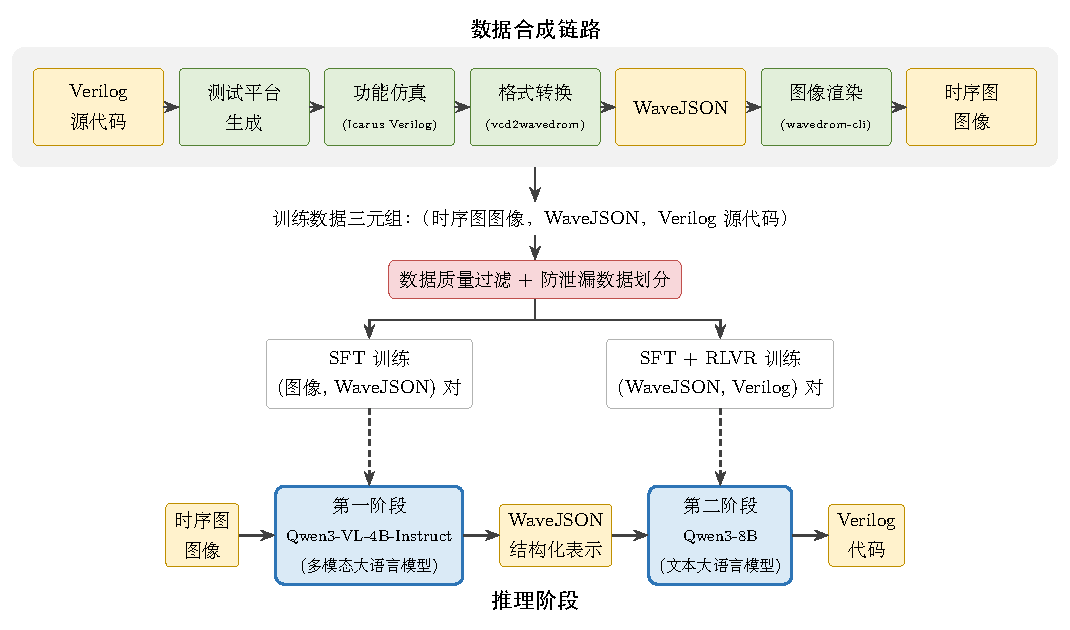
\includegraphics[width=\textwidth]{figures/framework.pdf}
  \caption{时序图自动化解析框架概览}
  \label{fig:framework}
\end{figure}

\textbf{第一阶段}采用多模态大语言模型Qwen3-VL-4B-Instruct实现图像到WaveJSON的转换，以时序图的PNG图像与文本提取指令作为输入，自回归地生成结构化表示。\textbf{第二阶段}采用纯文本大语言模型Qwen3-8B实现WaveJSON到Verilog代码的转换，以第一阶段的输出与生成指令作为输入，输出可综合的Verilog模块。

两阶段采用不同模型架构的考虑如下：第一阶段的核心挑战是跨模态视觉理解，需要多模态模型的图像感知能力；第二阶段的核心挑战是逻辑推理与代码生成，纯文本模型在此类任务上更具优势。同时，结构化中间表示使得两个阶段可以独立训练与优化，降低了端到端学习的难度。

整个框架的训练依赖大规模的配对数据：时序图图像与WaveJSON的配对用于第一阶段，WaveJSON与Verilog代码的配对用于第二阶段。高质量训练数据的匮乏是时序图解析任务面临的核心障碍。与自然图像或文档图像不同，数字电路时序图缺少现成的大规模标注数据集。TD-Interpreter\inlinecite{he2025tdinterpreter}率先提出了基于仿真的时序图数据合成思路，本文沿用这一基本思路。该链路以单个可综合Verilog模块的源代码为输入，经过以下四个步骤产出训练所需的三元组数据（时序图图像、WaveJSON结构化表示、Verilog源代码）：

\begin{enumerate}
  \item \textbf{测试平台生成。}为待测模块自动生成Verilog测试平台（Testbench），包含时钟驱动、输入激励序列与VCD波形转储语句。
  \item \textbf{功能仿真。}使用Icarus Verilog\inlinecite{williams2024iverilog}对模块源代码与测试平台进行联合编译与仿真，生成VCD（Value Change Dump）波形文件。
  \item \textbf{格式转换。}使用开源工具vcd2wavedrom\inlinecite{toroid2024vcd2wavedrom}将VCD文件转换为WaveJSON格式的结构化表示。
  \item \textbf{图像渲染。}使用wavedrom-cli\inlinecite{wavedrom2024cli}将WaveJSON渲染为SVG矢量图，再导出为PNG位图作为模型的视觉输入。
\end{enumerate}

在上述流程中，步骤2至4是确定性的工具链操作，合成数据的质量取决于两个关键因素：步骤1中测试平台的激励质量，以及对合成结果的质量筛选。本文分别在这两个维度上进行了系统性的改进，将在接下来的两节中详细介绍。


\section{测试平台生成策略}

测试平台的激励质量直接决定了仿真产生的波形是否包含有意义的信号行为模式。激励不足或缺乏功能语义的测试平台会导致波形退化为无意义的常量或噪声，严重影响训练数据的有效性。本文探索了两种测试平台生成方案：基于随机激励的基线方案与基于大语言模型的优化方案。


\subsection{基于随机激励的基线方案}

基线方案使用edautils工具包中的gentbvlog工具\inlinecite{edautils2024vlogtbgen}为Verilog模块自动生成测试平台。gentbvlog是一个基于Java的测试平台生成器，其工作流程为：解析Verilog模块的端口声明，识别时钟信号（按名称匹配\texttt{clk}或\texttt{clock}），为时钟信号生成固定频率的周期性驱动，为其余输入端口生成伪随机激励序列。

该方案的优势在于完全自动化且适用面广——只要Verilog模块语法正确，就能生成可仿真的测试平台。仿真运行时，时钟信号的最大仿真周期数被限制为20个，以控制生成时序图的长度。

然而，随机激励的固有局限也很明显：由于激励序列不具备任何功能语义，仿真产生的波形往往缺少有意义的信号行为模式。例如，一个有限状态机模块在随机输入下可能始终停留在复位状态，使得输出信号在整个仿真过程中保持常量不变。这类“退化”样本对模型训练的贡献有限，随机激励方案产生的低质量样本比例较高，限制了训练数据的有效规模。


\subsection{基于大语言模型的优化方案}

为克服随机激励缺乏功能语义的问题，本文引入大语言模型来生成具有工程意义的测试平台。该方案以随机激励方案的数据合成链路为基础，复用其仿真、格式转换与图像渲染等基础设施，仅替换测试平台生成环节。本文使用GPT-OSS-120B模型\inlinecite{openai2025gptoss}（一个1200亿参数的开源大语言模型）通过OpenAI兼容API进行测试平台生成，其核心思想是：将Verilog模块的源代码提供给LLM，令其分析模块功能后生成针对性的激励序列，使仿真产生的波形能够充分展示模块的各种工作状态。

本文设计了一套结构化的提示模板，要求LLM在生成测试平台时遵循以下关键规则：

\begin{enumerate}
  \item \textbf{DUT例化规范。}测试平台模块命名为\texttt{testbench}，将待测模块例化为\texttt{dut}（小写），端口连接必须与模块声明完全匹配。
  \item \textbf{初始化要求。}在\texttt{initial}块中将所有输入端口驱动至已知值，避免出现未定义状态（X态）。
  \item \textbf{时钟约束。}对含时钟的设计，使用\texttt{forever \#10 clk = \textasciitilde clk}生成20ns周期的时钟信号，仿真时间固定为400ns（20个完整时钟周期）。
  \item \textbf{激励分布约束。}要求激励序列在整个仿真时间窗口内均匀分布，至少在80\%的时钟周期内包含有意义的信号活动，避免激励集中在前几个周期而后续长时间空闲。
  \item \textbf{时序对齐。}所有信号变化必须发生在时钟沿或半周期整数倍时刻，禁止使用非整数延时（如\texttt{\#1}、\texttt{\#5}），以确保VCD到WaveJSON转换后波形的时间分辨率统一。
  \item \textbf{VCD转储。}测试平台中必须包含指定路径的\texttt{\$dumpfile}与\texttt{\$dumpvars}调用。
  \item \textbf{仿真终止。}使用独立的\texttt{initial}块在固定时刻调用\texttt{\$finish}，不在激励块中提前终止仿真。
\end{enumerate}

LLM的输出通过结构化标签（\texttt{<testbench\_verilog>}与\texttt{<skip\_reason>}）进行解析：若模型判断模块无法生成有效测试平台（如功能不明确），则返回跳过原因；否则返回完整的测试平台代码。

生成的测试平台经过与基线方案相同的后续流程——Icarus Verilog仿真、VCD转换、WaveJSON生成与图像渲染——最终产出训练数据三元组。相比随机激励方案，LLM生成的测试平台能够针对模块的具体功能设计有目的的激励序列：对有限状态机模块遍历各状态转移路径，对计数器模块测试边界溢出行为，对算术单元模块覆盖典型运算模式。这使得仿真产生的时序图包含更丰富、更具区分度的信号行为模式，从而为模型训练提供更高质量的监督信号。此外，具有功能覆盖性的测试平台在评估阶段同样发挥重要作用：如第~\ref{sec:sim-eval}~小节所述，第二阶段通过仿真对拍评估生成代码的功能正确性，激励序列越能覆盖模块的关键行为模式，对拍结果就越能有效区分功能正确与功能错误的生成代码。


\section{数据质量过滤}

除测试平台的激励质量外，对合成结果的质量筛选是保障训练数据有效性的另一关键维度。自动化合成的数据不可避免地包含低质量样本——如仿真失败产生的空白波形、尺寸畸形的图像、信号行为退化为常量的样本等——直接用于训练会引入噪声甚至误导模型。本文设计了贯穿数据合成全流程的多层级质量过滤机制，按作用阶段分为两个层次。

\subsection{Verilog源码预筛}

在进入仿真流程之前，对Verilog源文件进行以下检查，排除无法独立仿真的模块：
\begin{itemize}
  \item 排除含有\texttt{`include}指令的文件，因为其依赖外部文件无法独立仿真。
  \item 排除使用\texttt{\$readmemh}系统调用的文件，因为缺少外部数据文件。
  \item 排除标注了黑盒（\texttt{blackbox}）属性的模块。
  \item 排除不含任何行为描述（\texttt{always}块、\texttt{assign}连续赋值或门级原语实例化）的空壳模块。
  \item 使用Icarus Verilog进行语法检查，排除语法不正确的文件。
  \item 排除包含多个\texttt{module}定义的文件，确保每个数据样本对应单一的待测模块。
  \item 排除模块名匹配工艺库标准单元命名模式（如以\texttt{sky130}、\texttt{altera}、\texttt{xilinx}等为前缀）的模块，因为这些是工艺库原语而非可综合RTL设计。
\end{itemize}

该预筛同时适用于随机激励方案与LLM优化方案，是所有后续处理的前提条件。

\subsection{基于随机管线的仿真产出质量预选}

通过源码预筛的Verilog模块进入随机激励方案的数据合成管线。编译或仿真失败的模块不会产出VCD文件，自动排除在数据集之外。对成功产出时序图图像与WaveJSON的样本，进一步进行多维度的质量筛选：
\begin{itemize}
  \item \textbf{图像尺寸约束。}设置像素总数的上下界，排除过小（信息不足）或过大（超出模型处理能力）的图像。
  \item \textbf{宽高比约束。}限制图像宽高比在合理范围内，排除极端形状的图像。
  \item \textbf{信号数量约束。}限制WaveJSON中的信号数量，排除信号过少或过多的样本。
\end{itemize}

该筛选同时为LLM优化方案提供候选模块的预选。由于LLM API调用成本较高，本文利用随机管线的产出作为低成本的探针，先排除具有极端尺寸或形状的样本，仅将通过全部筛选的模块送入LLM管线，从而显著降低API调用开销。


\section{防泄漏数据划分}

在将过滤后的数据划分为训练集与测试集时，必须防止训练集与测试集之间的信息泄漏——即避免高度相似的样本同时出现在两个集合中，导致评估结果虚高。本文采用基于并查集（Disjoint Set Union, DSU）的防泄漏划分策略，通过多维度的相似性检测将相似样本归为同一等价类，确保同一等价类的所有样本被完整地分配到同一集合中。

相似性检测包含以下两个维度：
\begin{enumerate}
  \item \textbf{WaveJSON指纹匹配。}对每个样本计算其WaveJSON的规范化指纹：首先对所有信号名进行规范化（统一小写、去除空格、规范化总线索引格式），然后将每个信号的规范化名称与波形字符串组成二元组，按信号名排序后序列化为确定性字符串作为指纹。指纹相同的样本被归入同一等价类。
  \item \textbf{信号名模糊匹配。}在波形拓扑多重集（将波形字符串抽象为高/低/数据/保持等拓扑符号的多重集合）相同的样本之间，计算规范化信号名序列的相似度。相似度超过阈值（默认0.88）的样本对被合并。这一机制能够检测出仅因端口重命名而产生的变体样本。
\end{enumerate}

两个维度的检测结果通过并查集进行传递性合并，最终按等价类为单位进行训练/测试集的整组划分。


\section{评价指标}\label{sec:metrics}

在介绍模型训练方法之前，本文首先定义面向时序图结构化表示的专用评价指标。该指标既用于量化评估模型的解析质量，也将在后续强化学习阶段作为奖励函数发挥核心作用。

对于第一阶段（图像到WaveJSON），该指标直接将模型预测的WaveJSON与标准答案WaveJSON进行结构化比较。对于第二阶段（WaveJSON到Verilog代码），由于模型输出不再是WaveJSON，本文通过功能仿真将生成代码的行为转换回WaveJSON后再进行比较，具体方法将在第~\ref{sec:sim-eval}~小节介绍。

传统的文本相似度指标（如BLEU\inlinecite{papineni2002bleu}、ROUGE\inlinecite{lin2004rouge}）无法有效衡量WaveJSON解析结果的正确性。例如，两个WaveJSON在信号顺序不同但内容完全一致时，文本相似度会显著降低；而一个波形字符串中单个字符的错误可能导致后续所有时钟周期的语义偏移，但文本相似度的下降却不与语义损失成正比。因此，本文设计了面向WaveJSON结构特性的专用评价指标。

\subsection{信号匹配}

评价的第一步是建立预测结果与标准答案之间的信号对应关系。本文采用两阶段匹配策略：

\textbf{精确匹配阶段。}对预测与标准答案中的信号名进行规范化处理（统一大小写、去除空格、规范化总线索引格式），然后进行一对一的精确匹配。

\textbf{模糊匹配阶段。}对未在精确匹配阶段配对的信号，使用Levenshtein编辑距离\inlinecite{levenshtein1966binary}计算信号名之间的相似度。采用贪心策略，优先配对相似度最高的信号对，相似度低于阈值（默认0.7）的不予配对。

模糊匹配的引入是为了应对信号名的轻微变体（如\texttt{data\_out}与\texttt{dataout}），同时信号名匹配的相似度将作为后续波形评分的权重因子。

\subsection{波形评分}

对每对匹配的信号，本文在两种互补的粒度上评估波形的一致性。

\textbf{词元（Token）模式。}将波形字符串展开为逐周期的词元序列：保持字符（\texttt{.}）被替换为前一周期的实际状态值，数据字符（\texttt{=}）被替换为\texttt{data}数组中对应的标签文本。展开后的两条词元序列使用Levenshtein比率计算相似度，其定义为：
\begin{equation}
  \text{ratio}(s_1, s_2) = \frac{|s_1| + |s_2| - d(s_1, s_2)}{|s_1| + |s_2|}
\end{equation}
其中$d(s_1, s_2)$为两序列间的编辑距离。该模式关注逐周期的电平精确匹配。

\textbf{边沿（Edge）模式。}在展开的词元序列基础上提取沿签名（Edge Signature）：记录初始电平与每次电平跳变的位置和目标电平（例如\texttt{0:1}表示位置0的电平为高，\texttt{3:0}表示位置3跳变为低电平）。对两条沿签名序列同样使用Levenshtein比率计算相似度。该模式关注信号跳变的时序对齐，对时钟信号和边沿触发逻辑的评估更为敏感。

两种模式还针对WaveDrom时钟信号的表示特性进行了等价性处理：时钟信号既可以用专用字符（\texttt{p}表示上升沿、\texttt{n}表示下降沿）表示，也可以用\texttt{0}/\texttt{1}交替表示。评分时会枚举两种表示方式的所有初相组合，取最高分作为最终得分，避免因表示风格差异而产生不必要的扣分。

\subsection{综合评分}

对每个样本，将所有匹配信号对的波形得分（乘以信号名匹配的相似度权重）进行汇总，计算精确率（Precision）、召回率（Recall）与F1分数：
\begin{align}
  \text{Precision} &= \frac{\sum_{(g,p,s) \in M} s \cdot \text{WaveScore}(g, p)}{|P|} \\
  \text{Recall}    &= \frac{\sum_{(g,p,s) \in M} s \cdot \text{WaveScore}(g, p)}{|G|} \\
  \text{F1}        &= \frac{2 \cdot \text{Precision} \cdot \text{Recall}}{\text{Precision} + \text{Recall}}
\end{align}
其中$M$为匹配信号对集合，$(g, p, s)$分别为标准答案信号名、预测信号名与信号名匹配相似度，$\text{WaveScore}(g, p)$为对应的波形得分，$|G|$与$|P|$分别为标准答案与预测结果中的信号总数。

精确率衡量预测结果中有多大比例是正确的，召回率衡量标准答案中有多大比例被正确识别，F1分数是两者的调和平均。该指标从信号名的匹配准确性与波形序列的时序一致性两个层面对解析结果进行量化评估。

\subsection{基于仿真对拍的代码评估}\label{sec:sim-eval}

第二阶段的任务是从WaveJSON生成Verilog代码，其输出不再是WaveJSON结构，无法直接应用上述指标。本文采用基于功能仿真的对拍验证方法：将模型生成的Verilog模块与该样本对应的原始测试平台通过Icarus Verilog联合编译并运行仿真，将仿真产出的VCD波形转换为WaveJSON后，与标准答案WaveJSON进行上述指标的对比评分。

该方法不直接比较生成代码与参考代码的文本相似度，而是比较两者在相同激励下的功能行为是否一致。这一评估策略的合理性基于以下考虑：

\begin{enumerate}
  \item \textbf{功能等价性优于文本相似度。}数字电路设计中，功能等价的模块可以有截然不同的实现方式——同一个计数器既可以用\texttt{always}块的行为级描述实现，也可以用门级原语例化实现；同一个状态机的状态编码可以是二进制、格雷码或独热码。直接比较代码文本会将合理的实现差异误判为错误，而基于仿真的对拍验证关注的是输入-输出行为的一致性，与具体实现方式无关。
  \item \textbf{测试平台提供确定性的验证环境。}每个样本的测试平台在数据合成阶段已经生成并通过了仿真验证，其激励序列是固定的。将生成代码置于相同的测试平台下运行，保证了评估条件的一致性与可复现性。
  \item \textbf{评估粒度与任务目标对齐。}第二阶段的任务目标是从时序图的结构化表示还原出功能正确的Verilog模块。将生成模块的仿真波形与原始波形对拍，直接衡量的是“生成的模块是否复现了时序图所描述的信号行为”，与任务定义高度一致。
\end{enumerate}

需要指出的是，基于有限长度激励序列的仿真对拍是一种充分但非必要的功能验证——通过对拍的模块在所测试的输入序列上行为正确，但不能保证在所有可能输入下均正确。然而，本文数据集中的测试平台经过LLM针对性设计，激励序列覆盖了模块的主要工作模式与边界条件，在实践中提供了可靠的功能正确性评估。


\section{有监督微调}

\subsection{第一阶段：时序图图像到WaveJSON}

第一阶段使用Qwen3-VL-4B-Instruct\inlinecite{bai2025qwen3vl}作为基础模型，通过LoRA\inlinecite{hu2021lora}进行有监督微调。训练数据为时序图PNG图像与WaveJSON的配对，以ShareGPT多轮对话格式\inlinecite{chiang2023vicuna}组织：用户消息包含图像标记与提取指令，助手消息为对应的WaveJSON文本。

训练的关键超参数设置如下：
\begin{itemize}
  \item LoRA秩设为32，应用于模型的全部线性层。
  \item 冻结视觉编码器（Vision Tower）与多模态投影层的参数，仅训练语言模型部分的LoRA适配器。这一策略基于以下考虑：预训练的视觉编码器已具备充分的图像特征提取能力，时序图理解的瓶颈在于语言模型对视觉特征的解读方式，而非视觉特征本身的质量。
  \item 图像最大像素数限制为$1{,}048{,}576$（约$1024 \times 1024$），序列截断长度为8196个词元（Token）。
  \item 总批大小为64，学习率为$1 \times 10^{-4}$，使用恒定学习率调度，训练15轮（Epoch）。
\end{itemize}


\subsection{第二阶段：WaveJSON到Verilog代码}

第二阶段使用Qwen3-8B\inlinecite{yang2025qwen3}作为基础模型，同样通过LoRA进行有监督微调。训练数据为WaveJSON与Verilog模块源代码的配对：用户消息包含WaveJSON文本与生成指令，助手消息为对应的Verilog代码（已去除注释）。

训练的关键超参数设置如下：
\begin{itemize}
  \item LoRA秩设为64（高于第一阶段），因为代码生成任务的输出空间更大，需要更强的适配能力。应用于模型的全部线性层。
  \item 采用FSDP（Fully Sharded Data Parallel）\inlinecite{zhao2023fsdp}进行分布式训练，使用\texttt{full\_shard}策略，将模型参数、梯度与优化器状态分片存储于多块GPU上以降低单卡显存占用。
  \item 序列截断长度为8192个词元（Token）。
  \item 总批大小为64，学习率为$2 \times 10^{-5}$，使用恒定学习率调度，训练15轮（Epoch）。
\end{itemize}

两个阶段的训练均使用LlamaFactory框架\inlinecite{zheng2024llamafactory}完成，采用BF16混合精度训练以降低显存占用。


\section{基于强化学习的优化}

有监督微调使模型学会了从WaveJSON到Verilog代码的基本映射，但生成代码的功能正确性仍有提升空间。为此，本文引入基于可验证奖励的强化学习（Reinforcement Learning with Verifiable Rewards, RLVR）进行进一步优化。

\subsection{奖励函数设计}

RLVR的关键是设计可自动验证的奖励信号。对于第二阶段的WaveJSON到Verilog生成任务，本文利用功能仿真构建连续值奖励函数，其计算流程如下：

\begin{enumerate}
  \item \textbf{代码提取。}从模型的生成文本中解析Verilog代码段，优先提取代码围栏（Code Fence）内的内容，其次匹配\texttt{module}...\texttt{endmodule}结构。
  \item \textbf{模块名对齐。}将生成代码中声明的模块名重写为测试平台所期望的被测模块名称，确保仿真时模块实例化能够正确绑定。
  \item \textbf{功能仿真。}将对齐后的Verilog代码与对应的测试平台通过Icarus Verilog联合编译并运行，生成VCD波形文件。
  \item \textbf{波形对比评分。}将VCD文件转换为WaveJSON后，使用第~\ref{sec:metrics}~节描述的评价指标与标准WaveJSON进行对比，计算F1分数。
\end{enumerate}

最终奖励值直接取波形对比的F1分数，为$[0, 1]$区间内的连续值；若上述任一步骤失败（如编译错误、仿真超时），则奖励为零。连续值的奖励信号相比二值判定提供了更细粒度的优化梯度，使模型能够从部分正确的生成结果中获得正反馈。该奖励函数完全客观且可自动化执行，不依赖人工标注或主观判断，仅依赖确定性的仿真工具链与结构化的评分算法。

\subsection{GRPO优化}

本文采用群体相对策略优化（GRPO）\inlinecite{shao2024deepseekmath}算法进行强化学习训练，基于verl框架\inlinecite{sheng2024hybridflow}实现。对每个训练样本，模型采样一组候选Verilog代码，每份代码独立进行功能仿真与评分，所得F1分数作为该候选的奖励值。GRPO通过组内奖励的相对排名估计优势函数，消除了训练价值网络的额外开销。

训练数据与SFT阶段相同，将WaveJSON与对应的测试平台路径、参考Verilog代码等元信息打包为Parquet格式。强化学习阶段在SFT微调后的检查点上继续训练，关键超参数设置如下：
\begin{itemize}
  \item 沿用SFT阶段的LoRA配置：秩为64，缩放因子$\alpha$为128，应用于全部线性层。
  \item 对每个训练样本采样4个候选输出用于组内比较。
  \item 训练批大小为32，小批次大小为16，学习率为$3 \times 10^{-6}$。
  \item 禁用KL散度惩罚项，允许策略在仿真奖励的引导下自由探索。
  \item 使用vLLM\inlinecite{kwon2023vllm}作为推理引擎进行候选代码的批量生成，采用张量并行加速。
\end{itemize}

整个流程形成“生成—仿真—评分—更新”的闭环优化，逐步提升生成代码的功能正确性。
